%
% introduction.tex
%
% Copyright (C) 2022 by SpaceLab.
%
% Camera Payload Preliminary Design Review
%
% This work is licensed under the Creative Commons Attribution-ShareAlike 4.0
% International License. To view a copy of this license,
% visit http://creativecommons.org/licenses/by-sa/4.0/.
%

%
% \brief Introduction slides.
%
% \author Gabriel Mariano Marcelino <gabriel.mm8@gmail.com>
% \author Vitória Beatriz Bianchin <vitoriabbianchin@gmail.com>
% \author Caique Sales de Miranda Gomes <kiqsmg@gmail.com>
%
% \version 0.1.0
%
% \date 2022/06/24
%

\begin{frame}{Proposal and Objectives}
    
    \begin{columns}[t]
        \begin{column}[t]{0.65\textwidth}
            \begin{itemize}
                \item ADCS (Attitude Determination and Control System) Module
                \vspace{0.5cm}
                \item Project name: ``\textit{ADCS Module}''
                \vspace{0.5cm}
                \item Main objective: Create a module with basic instrumentation for an active magnetic ADCS system 
            \end{itemize}
        \end{column}
        \begin{column}[t]{0.4\textwidth}
            \begin{figure}[!ht]
                \begin{center}
                    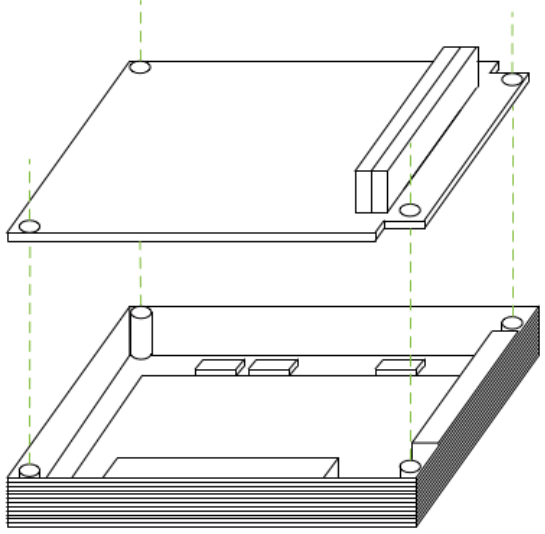
\includegraphics[width=4cm]{figures/adcs-module-idea.png}
                \end{center}
            \end{figure}
        \end{column}
    \end{columns}
    
\end{frame}

\begin{frame}{Requirements}

    \begin{itemize}
        \item \textbf{SLB-ADCS-REQ-001:} The module must be compliant with CubeSat and PC-104 standards; 
        \item \textbf{SLB-ADCS-REQ-002:} The module should be designed for 3U CubeSats (considering soft requirements for stabilization);
        \item \textbf{SLB-ADCS-REQ-003:} The module must include compact magnetic coils on 3-axis;
        \item \textbf{SLB-ADCS-REQ-004:} The module must have a microcontroller with sufficient performance for basic ADCS algorithms;  
        \item \textbf{SLB-ADCS-REQ-005:} The module must include built-in sensors: magnetometer (3-axis), gyroscope (3-axis), voltage/current (each coil), temperature (each coil), and sun sensor (photodiode interfaces for 3-axis); 
    \end{itemize}

\end{frame}

\begin{frame}{Requirements}

    \begin{itemize}
        \item \textbf{SLB-ADCS-REQ-006:} The module must have current (H-bridge) drivers with a safe operation for the magnetic coils;  
        \item \textbf{SLB-ADCS-REQ-007:} The module should assume moderate power consumption during stabilization;
        \item \textbf{SLB-ADCS-REQ-008:} The power circuits must have overcurrent/overvoltage/overtemperature protection (fuses, load switches, overtemperature shutdown, ...); 
        \item \textbf{SLB-ADCS-REQ-009:} The board should be designed to minimize overheating elements and mixing digital/analog/power circuits;    
        \item \textbf{SLB-ADCS-REQ-010:} The board should have 4 layers, including continuous power planes for better electrical/heat/noise performance.
    \end{itemize}

\end{frame}